% Created 2017-04-05 Wed 20:21
% Intended LaTeX compiler: pdflatex
\documentclass[a4paper,11pt]{article}
\usepackage[utf8]{inputenc}
\usepackage[T1]{fontenc}
\usepackage{graphicx}
\usepackage{grffile}
\usepackage{longtable}
\usepackage{wrapfig}
\usepackage{rotating}
\usepackage[normalem]{ulem}
\usepackage{amsmath}
\usepackage{textcomp}
\usepackage{amssymb}
\usepackage{capt-of}
\usepackage{hyperref}
\usepackage[margin=1.2in]{geometry}
\usepackage{setspace}
\singlespacing
\usepackage{parskip}
\author{Zheng Tian}
\date{\today}
\title{}
\hypersetup{
 pdfauthor={Zheng Tian},
 pdftitle={},
 pdfkeywords={},
 pdfsubject={},
 pdfcreator={Emacs 25.1.1 (Org mode 9.0.3)},
 pdflang={English}}
\begin{document}

\tableofcontents

This file include answers and R codes for completing Empirical
Exercise 4.2 in Introduction to Econometrics (3rd edition) by Stock
and Watson.

\section{Reading the Data}
\label{sec:org27fea18}

The first step is to read the data file into R. The data files for
this problem are \texttt{TeachingRatings.dta} and \texttt{TeachingRatings.xls},
accompanied by a descriptive file \texttt{TeachingRatings\_Description.pdf}.

\begin{itemize}
\item Read the STATA file

\begin{verbatim}
library(foreign)
teachingdata <- read.dta("TeachingRatings.dta")
\end{verbatim}

\item Upon reading the data, we can take a glimpse on the data.

\begin{itemize}
\item Use \texttt{head} or \texttt{tail} to look at the first or last few observations

\begin{verbatim}
head(teachingdata)
\end{verbatim}
\end{itemize}
\end{itemize}


\section{Summary Statistics}
\label{sec:org73693f3}

We get the summary statistics of the variables used in the analysis,
which is \texttt{course\_eval} and \texttt{beauty}

\begin{verbatim}
df <- teachingdata[c("course_eval", "beauty")]
sumdf <- summary(df); sumdf
\end{verbatim}

\begin{verbatim}
 course_eval        beauty
Min.   :2.100   Min.   :-1.45049
1st Qu.:3.600   1st Qu.:-0.65627
Median :4.000   Median :-0.06801
Mean   :3.998   Mean   : 0.00000
3rd Qu.:4.400   3rd Qu.: 0.54560
Max.   :5.000   Max.   : 1.97002
\end{verbatim}

We can create a table that looks professional using \texttt{stargazer()}.
\begin{verbatim}
library(stargazer)
stargazer(df, type = "latex",
  title = "Summary Statistics", label = "tab:sum-stats")
\end{verbatim}


% Table created by stargazer v.5.2 by Marek Hlavac, Harvard University. E-mail: hlavac at fas.harvard.edu
% Date and time: Wed, Apr 05, 2017 - 20:20:56
\begin{table}[!htbp] \centering
  \caption{Summary Statistics}
  \label{tab:sum-stats}
\begin{tabular}{@{\extracolsep{5pt}}lccccc}
\\[-1.8ex]\hline
\hline \\[-1.8ex]
Statistic & \multicolumn{1}{c}{N} & \multicolumn{1}{c}{Mean} & \multicolumn{1}{c}{St. Dev.} & \multicolumn{1}{c}{Min} & \multicolumn{1}{c}{Max} \\
\hline \\[-1.8ex]
course\_eval & 463 & 3.998 & 0.555 & 2.100 & 5.000 \\
beauty & 463 & 0.00000 & 0.789 & $-$1.450 & 1.970 \\
\hline \\[-1.8ex]
\end{tabular}
\end{table}


\section{Scatterplot}
\label{sec:orgefbbadd}

We can make scatterplot using the \texttt{plot} function.

\begin{verbatim}
teaching.formula <- course_eval ~ beauty
plot(teaching.formula, data = teachingdata,
   main = "The Scatterplot of Course Evaluation on Professor's Beauty",
   xlab="Beauty", ylab = "Course evaluation", col = "blue")
\end{verbatim}

\begin{figure}[htbp]
\centering
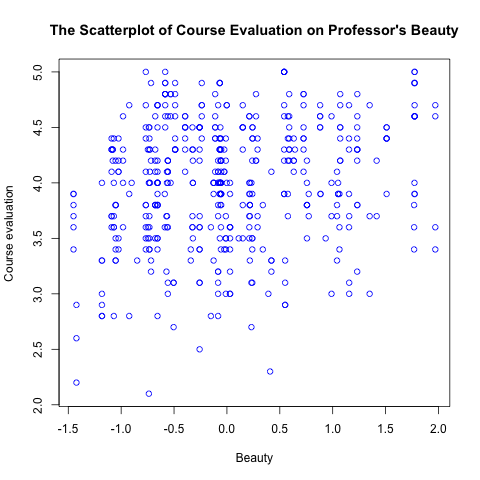
\includegraphics[width=0.75\textwidth]{beauty.png}
\caption{\label{fig:org08f2500}
The scatterplot of course evaulation on professors' beauty}
\end{figure}


\section{Regression}
\label{sec:org554f9f0}

Now let's estimate the regression model. The results is reported
in Table \ref{tab:ols-1}

\begin{verbatim}
# run a regression of course evaluation on professor's beauty
teaching.ols <- lm(teaching.formula, data = teachingdata)

# create the latex table
stargazer(teaching.ols,
  covariate.labels = c("Beauty"),
  dep.var.labels = c("Course Evaluations"),
  title = "The OLS Estimation of the Regression of Course Evaluation on Beauty",
  label = "tab:ols-1", single.row = TRUE, omit.stat = c("adj.rsq", "f")
)
\end{verbatim}


% Table created by stargazer v.5.2 by Marek Hlavac, Harvard University. E-mail: hlavac at fas.harvard.edu
% Date and time: Wed, Apr 05, 2017 - 20:20:56
\begin{table}[!htbp] \centering
  \caption{The OLS Estimation of the Regression of Course Evaluation on Beauty}
  \label{tab:ols-1}
\begin{tabular}{@{\extracolsep{5pt}}lc}
\\[-1.8ex]\hline
\hline \\[-1.8ex]
 & \multicolumn{1}{c}{\textit{Dependent variable:}} \\
\cline{2-2}
\\[-1.8ex] & Course Evaluations \\
\hline \\[-1.8ex]
 Beauty & 0.133$^{***}$ (0.032) \\
  Constant & 3.998$^{***}$ (0.025) \\
 \hline \\[-1.8ex]
Observations & 463 \\
R$^{2}$ & 0.036 \\
Residual Std. Error & 0.545 (df = 461) \\
\hline
\hline \\[-1.8ex]
\textit{Note:}  & \multicolumn{1}{r}{$^{*}$p$<$0.1; $^{**}$p$<$0.05; $^{***}$p$<$0.01} \\
\end{tabular}
\end{table}



\section{Answers to the questions}
\label{sec:org242dd1c}

\begin{description}
\item[{a.}] The scatterplot is Figure \ref{fig:org08f2500}. There appears to be
a weak positive relationship between course evaluation and the
beauty index.

\item[{b.}] The estimation results are reported in Table \ref{tab:ols-1}.

\begin{verbatim}
beauty.watson <- mean(teachingdata$beauty)
beauty.stock <- mean(teachingdata$beauty) + sd(teachingdata$beauty)
ave.courseval <- mean(teachingdata$course_eval)

# do prediction step by step
b0 <- teaching.ols$coef[1]
b1 <- teaching.ols$coef[2]
courseval.predict <- b0 + b1 * c(beauty.watson, beauty.stock)
names(courseval.predict) <- c("waston", "stock")
\end{verbatim}

The slope is \texttt{0.133} and the intercept is
\texttt{3.998}. The sample mean of course evaluation is
\texttt{3.998}, which coincides with the slope
because the sample mean of \emph{Beauty} is
\texttt{0}.
\end{description}


\begin{description}
\item[{c.}] The beauty indices for Professors Stock and Watson are
\texttt{0.7886} (one standard deviation)
and \texttt{0} (sample average).
Thus, the predicted course evaluations for Professors
Stock and Watson are \texttt{4.1032} and
\texttt{3.9983}, respectively.

\begin{verbatim}
beauty.sd <- sd(teachingdata$beauty)
courseval.sd <- sd(teachingdata$course_eval)
delta.courseval <- b1 * beauty.sd
\end{verbatim}

\item[{d.}] The standard deviation of course evaluation is
\texttt{0.5549}, and the standard deviation of
beauty is \texttt{0.7886}. A one-standard-deviation
increase in beauty is expected to increase course evaluation
by \texttt{0.1049}, or
\texttt{0.19} of standard deviation of course
evaluations. The effect is small.

\begin{verbatim}
rsq <- summary(teaching.ols)$r.squared
\end{verbatim}

\item[{e.}] The regression R\(^{\text{2}}\) is \texttt{0.0357}, so that \emph{Beauty}
explains only \texttt{3.6} percent of the
variance in course evaluations.
\end{description}
\end{document}